\documentclass[12pt,a4paper]{article}

\usepackage[utf8]{inputenc}
\usepackage[T1]{fontenc}
\usepackage[french]{babel}
\usepackage{graphicx}
\usepackage{geometry}
\usepackage{fancyhdr}
\usepackage{titlesec}
\usepackage{booktabs}
\usepackage{longtable}
\usepackage{array}
\usepackage{hyperref}
\usepackage{xcolor}
\usepackage{listings}
\usepackage{float}
\usepackage{caption}
\usepackage{subcaption}
\usepackage{amsmath}
\usepackage{enumitem}
\usepackage{tocloft}
\usepackage{tabularx}
\usepackage[export]{adjustbox}

\geometry{
    left=2.5cm,
    right=2.5cm,
    top=2.5cm,
    bottom=2.5cm
}

\hypersetup{
    colorlinks=true,
    linkcolor=black,
    urlcolor=blue,
    citecolor=black
}

\renewcommand{\lstlistingname}{Code}
\renewcommand{\lstlistlistingname}{Liste des Codes}
\lstset{
    backgroundcolor=\color{gray!10},
    basicstyle=\ttfamily\scriptsize,
    keywordstyle=\color{blue!70!black}\bfseries,
    commentstyle=\color{green!50!black}\itshape,
    stringstyle=\color{red!70!black},
    breaklines=true,
    breakatwhitespace=false,
    breakautoindent=true,
    postbreak=\mbox{\textcolor{red}{$\hookrightarrow$}\space},
    numbers=left,
    numberstyle=\tiny\color{gray},
    frame=single,
    rulecolor=\color{gray},
    captionpos=b,
    showstringspaces=false,
    tabsize=2,
    columns=flexible,
    keepspaces=true,
    xleftmargin=0.5cm,
    xrightmargin=0.5cm,
    linewidth=\linewidth
}

\pagestyle{fancy}
\fancyhf{}
\fancyhead[L]{\footnotesize INF438 - Bases de Données Avancées}
\fancyhead[R]{\footnotesize Groupe 3}
\fancyfoot[C]{\thepage}
\renewcommand{\headrulewidth}{0.4pt}
\renewcommand{\footrulewidth}{0.4pt}

\titleformat{\section}
    {\newpage\Large\bfseries}
    {\thesection.}{0.5em}{}
\titleformat{\subsection}
    {\large\bfseries}
    {\thesubsection}{0.5em}{}
\titleformat{\subsubsection}
    {\normalsize\bfseries}
    {\thesubsubsection}{0.5em}{}

\captionsetup[table]{name=Tableau}

\setcounter{tocdepth}{2}
\renewcommand{\contentsname}{TABLE DES MATIÈRES}
\renewcommand{\listfigurename}{LISTE DES FIGURES}
\renewcommand{\listtablename}{LISTE DES TABLEAUX}

\renewcommand{\arraystretch}{1.2}

\begin{document}

\begin{titlepage}
    \centering
    
    \vspace*{0.5cm}

    \includegraphics[max width=5cm, max height=5cm, keepaspectratio]{../Screenshots/Picture1}
    
    \vspace{1cm}
    
    {\Large\textbf{UNIVERSITÉ GALATASARAY}}\\[0.3cm]
    {\large Faculté d'Ingénierie et de Technologie}\\[0.3cm]
    {\large Département d'Informatique}
    
    \vspace{1.5cm}
    
    {\LARGE\textbf{INF438}}\\[0.3cm]
    {\Large\textbf{BASES DE DONNÉES AVANCÉES}}
    
    \vspace{1.5cm}
    
    \rule{\textwidth}{1.5pt}\\[0.5cm]
    {\Huge\textbf{Projet Final}}\\[0.3cm]
    {\Large Analyse E-Sport (Dota 2) sur}\\[0.2cm]
    {\Large Architecture Lakehouse Azure}\\[0.5cm]
    \rule{\textwidth}{1.5pt}
    
    \vspace{1.5cm}
    
    {\large\textbf{GROUPE 3}}
    
    \vspace{0.8cm}
    
    \begin{tabular}{rl}
        \textbf{Membre 1 :} & Sabri Taner Burak ALTINDAL -- 22401030 \\[0.2cm]
        \textbf{Membre 2 :} & Emirhan Karatepe -- 19401830 \\[0.2cm]
        \textbf{Membre 3 :} & Kaan Çolakoğlu -- 21401946 \\[0.2cm]
        \textbf{Membre 4 :} & Ceren Akbaş -- 22401028 \\
    \end{tabular}
    
    \vfill
    
    {\large\textbf{Année Académique 2025--2026}}

\end{titlepage}

\newpage
\tableofcontents
\newpage

\listoffigures
\newpage

\listoftables
\newpage

% Section 1: Introduction
\section{Introduction}

\subsection{Contexte du Projet}

L'industrie de l'e-sport a connu une croissance exponentielle au cours de la dernière décennie, devenant aujourd'hui un écosystème de plusieurs milliards de dollars. Avec cette croissance, la quantité de données générées lors des tournois professionnels a également augmenté de manière significative. L'analyse des performances des joueurs, l'optimisation des stratégies d'équipe et la prédiction des résultats des matchs sont des domaines critiques où l'ingénierie des données et la science des données trouvent des applications pratiques.

Dans le cadre de ce projet, une solution complète d'ingénierie des données a été conçue et implémentée pour le traitement, l'analyse et le développement de modèles prédictifs sur les données des matchs professionnels de Dota 2. Le projet a été réalisé sur la plateforme Microsoft Azure, en adoptant les principes modernes d'architecture cloud.

\subsection{Jeu de Données Utilisé}

Le jeu de données utilisé dans ce projet est le \textbf{``Dota 2 Pro League Matches 2023''} publié sur la plateforme Kaggle. Ce jeu de données contient des enregistrements détaillés des matchs des tournois professionnels de Dota 2 tout au long de l'année 2023.

\begin{table}[H]
\centering
\caption{Caractéristiques du jeu de données}
\label{tab:dataset}
\begin{tabular}{>{\centering\arraybackslash}m{4cm}>{\centering\arraybackslash}m{2cm}>{\centering\arraybackslash}m{5cm}}
\toprule
\textbf{Nom du Fichier} & \textbf{Taille} & \textbf{Description} \\
\midrule
main\_metadata.csv & 9.09 MB & Métadonnées des matchs \\
players\_reduced.csv & 152.00 MB & Statistiques des joueurs \\
picks\_bans.csv & 33.01 MB & Données de sélection/bannissement \\
teams.csv & 8.09 MB & Informations sur les équipes \\
\bottomrule
\end{tabular}
\end{table}

Le format CSV et la structure relationnelle du jeu de données ont nécessité un processus complet de nettoyage et de fusion lors de la transition de la couche Bronze vers la couche Silver.

\subsection{Objectifs du Projet}

Les objectifs principaux de ce projet ont été définis comme suit :

\begin{enumerate}[label=\arabic*.]
    \item \textbf{Mise en place de l'Architecture Lakehouse :} Implémentation de la Medallion Architecture (Bronze-Silver-Gold) sur Azure Data Lake Storage Gen2
    \item \textbf{Pipeline de Traitement Batch :} Création de pipelines ETL automatisés utilisant Azure Data Factory et Databricks
    \item \textbf{Simulation de Streaming :} Développement d'un simulateur imitant le flux de données en temps réel
    \item \textbf{Transformation des Données :} Transformation des données brutes en tables analytiques à l'aide de PySpark
    \item \textbf{Analyse Avancée :} Analyses de performance des joueurs et des héros avec SQL et PySpark
    \item \textbf{Machine Learning :} Développement d'un modèle de prédiction des résultats de matchs et suivi avec MLflow
\end{enumerate}

\subsection{Services Azure Utilisés}

\begin{table}[H]
\centering
\caption{Services Microsoft Azure utilisés}
\label{tab:azure-services}
\begin{tabular}{>{\centering\arraybackslash}m{5cm}>{\centering\arraybackslash}m{7cm}}
\toprule
\textbf{Service} & \textbf{Objectif d'Utilisation} \\
\midrule
Azure Data Lake Storage Gen2 & Stockage central pour les couches Lakehouse \\
Azure Data Factory & Orchestration des pipelines et planification \\
Azure Databricks & Traitement des données et développement ML \\
Delta Lake & Format de données performant conforme ACID \\
MLflow & Suivi des expériences de machine learning \\
Power BI & Visualisation et création de tableaux de bord \\
\bottomrule
\end{tabular}
\end{table}

Toutes les ressources ont été créées à l'aide de l'abonnement \textbf{Microsoft Azure for Students} et gérées en tenant compte de l'optimisation des coûts.

% Section 2: Conception Architecturale
\section{Conception Architecturale}

\subsection{Medallion Architecture}

Dans ce projet, la \textbf{Medallion Architecture} (Architecture Médaillon), largement adoptée dans les pratiques modernes d'ingénierie des données, a été appliquée. Cette architecture divise les données en trois couches selon leur niveau de qualité et de traitement : \textbf{Bronze}, \textbf{Silver} et \textbf{Gold}.

\subsubsection{Couche Bronze (Données Brutes)}

La couche Bronze est la couche où les données provenant des systèmes sources sont stockées telles quelles, sans aucune transformation :

\begin{itemize}
    \item \textbf{Objectif :} Conservation d'une copie exacte de la source de données
    \item \textbf{Format :} CSV et JSON (pour la simulation de streaming)
    \item \textbf{Contenu :} 4 fichiers CSV principaux + fichiers JSON de streaming
    \item \textbf{Utilisation :} Retour à la source en cas d'erreur, audit et traçabilité
\end{itemize}


\subsubsection{Couche Silver (Données Nettoyées)}

La couche Silver est la couche intermédiaire où les données brutes sont nettoyées et standardisées :

\begin{itemize}
    \item \textbf{Objectif :} Fournir des données propres et cohérentes
    \item \textbf{Format :} Delta Lake (basé sur Parquet)
    \item \textbf{Transformations :} Nettoyage des valeurs nulles, standardisation des types, élimination des doublons, détection d'outliers
\end{itemize}

\begin{table}[H]
\centering
\caption{Tables de la couche Silver}
\label{tab:silver-tables}
\begin{tabular}{>{\centering\arraybackslash}m{5cm}>{\centering\arraybackslash}m{5cm}}
\toprule
\textbf{Table} & \textbf{Nombre d'Enregistrements} \\
\midrule
cleaned\_matches & 29 809 \\
cleaned\_players & 8 456 \\
cleaned\_picks\_bans & 710 414 \\
\bottomrule
\end{tabular}
\end{table}

\subsubsection{Couche Gold (Données Analytiques)}

La couche Gold contient les données enrichies avec la logique métier :

\begin{table}[H]
\centering
\caption{Tables de la couche Gold}
\label{tab:gold-tables}
\begin{tabular}{>{\centering\arraybackslash}m{4.5cm}>{\centering\arraybackslash}m{4.5cm}>{\centering\arraybackslash}m{3cm}}
\toprule
\textbf{Table} & \textbf{Description} & \textbf{Enregistrements} \\
\midrule
esports\_gold.player\_stats & Métriques de performance & 813 \\
esports\_gold.hero\_stats & Statistiques des héros & 123 \\
esports\_gold.daily\_stats & Statistiques quotidiennes & 365 \\
esports\_gold.ml\_features & Features pour le ML & 8 312 \\
\bottomrule
\end{tabular}
\end{table}

\subsection{Structure Azure Data Lake Storage Gen2}

Toutes les couches Lakehouse sont positionnées sur Azure Data Lake Storage Gen2 :

\begin{itemize}
    \item \textbf{Storage Account :} \texttt{dota2lakehousenew}
    \item \textbf{Container :} \texttt{data}
    \item \textbf{Chemins :}
    \begin{itemize}
        \item Bronze : \texttt{abfss://data@dota2lakehousenew.../bronze/}
        \item Silver : \texttt{abfss://data@dota2lakehousenew.../silver/}
        \item Gold : \texttt{abfss://data@dota2lakehousenew.../gold/}
    \end{itemize}
\end{itemize}

\begin{figure}[H]
\centering
\includegraphics[max width=\textwidth, max height=0.75\textheight, keepaspectratio]{../Screenshots/Picture2}
\caption{Vue Azure Portal de la structure des dossiers Bronze/Silver/Gold dans ADLS Gen2}
\label{fig:adls-structure}
\end{figure}

\subsection{Diagramme de Flux de Données}

Le flux de données de bout en bout du système suit le parcours suivant : les données sources provenant de Kaggle et du simulateur de streaming sont d'abord stockées dans la couche Bronze. Ensuite, Azure Data Factory orchestre les notebooks Databricks qui transforment les données vers les couches Silver puis Gold. Enfin, les données Gold alimentent les analyses SQL, le modèle de machine learning (suivi par MLflow), et les visualisations Power BI.

\begin{figure}
    \centering
    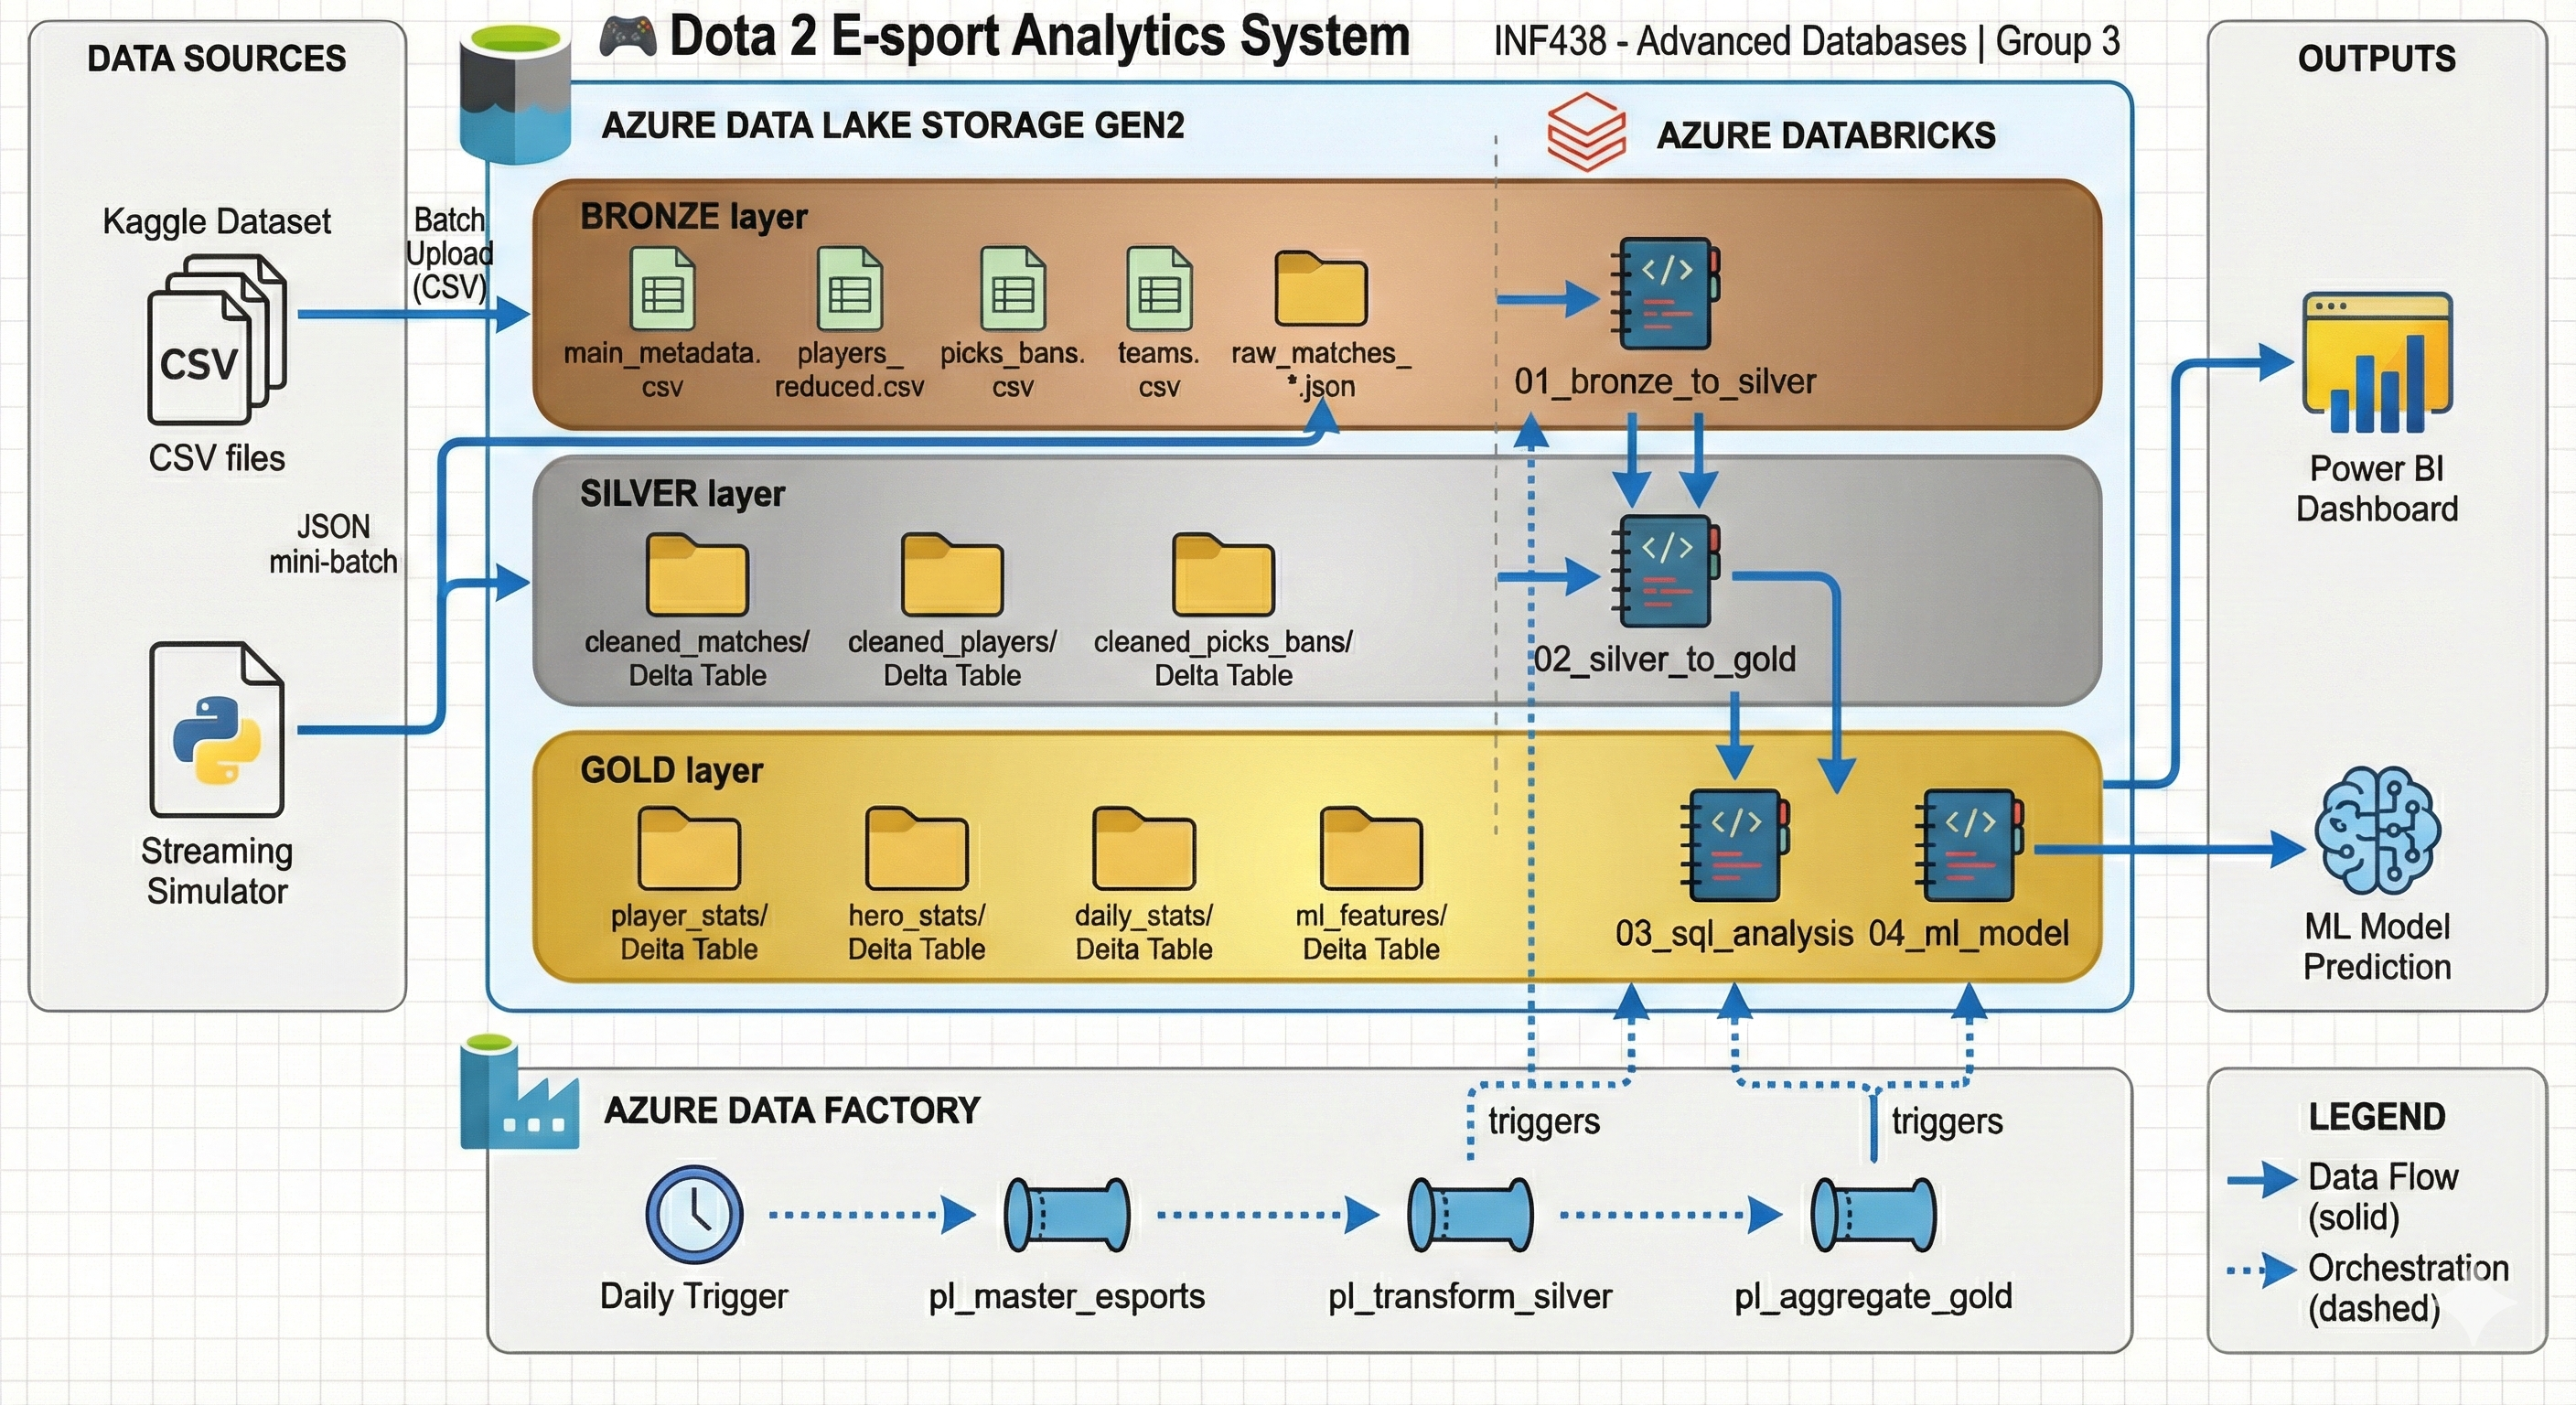
\includegraphics[width=0.60\linewidth]{../Screenshots/pipeline.png}
    \caption{Diagramme de flux de donnees}
    \label{fig:placeholder}
\end{figure}

% Section 3: Implémentation
\section{Implémentation}

\subsection{Pipeline de Traitement Batch}

Azure Data Factory (ADF) a été utilisé pour l'orchestration du pipeline de traitement batch. Le pipeline principal créé dans le projet porte le nom \textbf{pl\_master\_esports}.

En amont de ce traitement, un pipeline d'ingestion spécifique nommé \\\texttt{PL\_Ingest\_Kaggle\_To\_Bronze} a été mis en place. Ce pipeline utilise une activité \textit{Copy Data} pour transférer automatiquement les fichiers bruts (CSV) et le jeu de données réduit vers le conteneur \texttt{bronze/} du Data Lake, assurant ainsi la disponibilité des données pour les notebooks Databricks.

\begin{figure}[H]
\centering
\includegraphics[max width=\textwidth, max height=0.75\textheight, keepaspectratio]{../Screenshots/batch_pipeline.png}
\caption{Détails d'exécution de l'activité \textit{Copy Data} confirmant l'ingestion réussie des 4 fichiers sources (212 MB) vers le conteneur Bronze.}
\label{fig:adf-pipeline}
\end{figure}

La structure du pipeline est conçue comme suit :
\begin{itemize}
    \item \textbf{Activité 1 :} nb\_bronze\_to\_silver (Databricks Notebook)
    \item \textbf{Activité 2 :} nb\_silver\_to\_gold (dépend de l'Activité 1)
    \item \textbf{Activité 3 :} nb\_ml\_model (dépend de l'Activité 2)
\end{itemize}

\begin{figure}[H]
\centering
\includegraphics[max width=\textwidth, max height=0.75\textheight, keepaspectratio]{../Screenshots/Picture3}
\caption{Diagramme du pipeline pl\_master\_esports dans Azure Data Factory}
\label{fig:adf-pipeline}
\end{figure}

\subsection{Configuration du Déclencheur}

Un déclencheur nommé \textbf{tr\_daily\_esports} a été créé pour l'exécution automatique du pipeline.

\begin{table}[H]
\centering
\caption{Configuration du trigger}
\label{tab:trigger-config}
\begin{tabular}{>{\centering\arraybackslash}m{4cm}>{\centering\arraybackslash}m{5cm}}
\toprule
\textbf{Paramètre} & \textbf{Valeur} \\
\midrule
Nom du Trigger & tr\_daily\_esports \\
Type & Schedule Trigger \\
Fréquence & Quotidien (Daily) \\
Heure de Début & 02:00 UTC \\
État & Actif \\
\bottomrule
\end{tabular}
\end{table}

\begin{figure}[H]
\centering
\includegraphics[max width=\textwidth, max height=0.75\textheight, keepaspectratio]{../Screenshots/Picture4}
\caption{État ``Succeeded'' et ``Triggered by tr\_daily\_esports'' dans l'écran ADF Monitor}
\label{fig:adf-monitor}
\end{figure}

\subsection{Notebooks Databricks}

Les opérations de transformation des données ont été réalisées en utilisant PySpark sur Azure Databricks.

\begin{table}[H]
\centering
\caption{Configuration du cluster Databricks}
\label{tab:cluster-config}
\begin{tabular}{>{\centering\arraybackslash}m{4cm}>{\centering\arraybackslash}m{5cm}}
\toprule
\textbf{Paramètre} & \textbf{Valeur} \\
\midrule
Mode du Cluster & Standard \\
Type de Nœud & Standard\_DS3\_v2 \\
Auto Termination & 120 minutes \\
Databricks Runtime & 13.3 LTS (Spark 3.4.1) \\
\bottomrule
\end{tabular}
\end{table}

\textbf{Notebooks créés :}
\begin{enumerate}
    \item \textbf{setup\_connection.ipynb} : Test de connexion Azure ADLS Gen2
    \item \textbf{01\_bronze\_to\_silver.ipynb} : Nettoyage des données brutes
    \item \textbf{02\_silver\_to\_gold.ipynb} : Application de la logique métier
    \item \textbf{04\_ml\_model.ipynb} : Entraînement du modèle ML
\end{enumerate}

Le code source complet de ces notebooks est disponible en \textbf{Annexe~\ref{appendix:notebooks}}.

\subsection{Simulation de Streaming}

En l'absence d'une source de données en temps réel, un script Python simulant le comportement de streaming a été développé. Le script \textbf{stream\_simulator.py} fonctionne selon la logique suivante :

\begin{enumerate}
    \item Les enregistrements sont lus à partir du fichier main\_metadata.csv
    \item Les enregistrements sont divisés en mini-batches de 5
    \item Un délai artificiel de 3 secondes est appliqué pour chaque mini-batch
    \item Le mini-batch est nommé avec un timestamp unique et écrit dans Bronze
\end{enumerate}

\begin{figure}[H]
\centering
\includegraphics[max width=\textwidth, max height=0.75\textheight, keepaspectratio]{../Screenshots/simulation-streaming.png}
\caption{Sortie d'exécution du code stream\_simulator.py}
\label{fig:stream-output}
\end{figure}

Lorsque le simulateur est exécuté, des fichiers sont créés dans la couche Bronze avec le format \texttt{raw\_matches\_YYYYMMDD\_HHMMSS.json} (10 fichiers au total).

Le code source complet du simulateur est disponible en \textbf{Annexe~\ref{appendix:streaming}}.

\subsection{Transformations ETL}

\subsubsection{Transformation Bronze → Silver}

Les données CSV brutes de la couche Bronze ont subi un processus de transformation complet :

\begin{itemize}
    \item \textbf{Chargement :} Lecture des fichiers CSV avec inférence de schéma
    \item \textbf{Nettoyage :} Suppression des colonnes inutiles, filtrage des valeurs nulles
    \item \textbf{Validation :} Filtrage des matchs avec durée invalide ($<$5 min ou $>$2 heures)
    \item \textbf{Enrichissement :} Création de nouvelles features (duration\_minutes, kda\_calculated)
    \item \textbf{Détection d'outliers :} Marquage avec la règle des 3 sigma
\end{itemize}

\subsubsection{Transformation Silver → Gold}

Les données nettoyées ont reçu une logique métier et des calculs avancés.

\textbf{Statistiques des Joueurs (player\_stats) :} Agrégation par compte joueur avec calcul des moyennes (KDA, GPM, XPM) et du taux de victoire. Résultat : statistiques calculées pour \textbf{813 joueurs uniques}.

\textbf{Analyse Méta des Héros (hero\_stats) :} Un algorithme de classification des héros en 5 tiers selon leur taux de présence (voir Tableau~\ref{tab:tier-criteria}).

\begin{table}[H]
\centering
\caption{Critères de classification Meta Tier}
\label{tab:tier-criteria}
\begin{tabular}{>{\centering\arraybackslash}m{3cm}>{\centering\arraybackslash}m{5cm}}
\toprule
\textbf{Tier} & \textbf{Critère de Presence Rate} \\
\midrule
S-Tier & $>$ 50\% \\
A-Tier & $>$ 30\% \\
B-Tier & $>$ 15\% \\
C-Tier & $>$ 5\% \\
D-Tier & $\leq$ 5\% \\
\bottomrule
\end{tabular}
\end{table}

\begin{figure}[H]
\centering
\includegraphics[max width=\textwidth, max height=0.75\textheight, keepaspectratio]{../Screenshots/Picture6}
\caption{Sortie de la classification Tier dans le notebook silver\_to\_gold}
\label{fig:tier-classification}
\end{figure}

\textbf{Analyse de la Durée des Matchs :}

\begin{table}[H]
\centering
\caption{Résultats de l'analyse de durée}
\label{tab:duration-analysis}
\begin{tabular}{>{\centering\arraybackslash}m{3.5cm}>{\centering\arraybackslash}m{2cm}>{\centering\arraybackslash}m{2cm}>{\centering\arraybackslash}m{2.5cm}}
\toprule
\textbf{Durée} & \textbf{Matchs} & \textbf{Avg Kills} & \textbf{Radiant Win} \\
\midrule
Very Short ($<$25min) & 4 176 & 44.94 & 53.54\% \\
Short (25-35min) & 13 548 & 56.74 & 50.41\% \\
Medium (35-45min) & 8 162 & 65.33 & 49.36\% \\
Long (45-55min) & 2 839 & 68.19 & 49.52\% \\
Very Long ($>$55min) & 1 084 & 80.77 & 50.46\% \\
\bottomrule
\end{tabular}
\end{table}

\subsection{Gestion des Tables Delta Lake}

Les tables de la couche Gold sont gérées sous le schéma \textbf{esports\_gold} dans le Databricks Unity Catalog. Les commandes SQL de création sont disponibles en \textbf{Annexe~\ref{appendix:sql}}.

\begin{figure}[H]
\centering
\includegraphics[max width=\textwidth, max height=0.75\textheight, keepaspectratio]{../Screenshots/Picture7}
\caption{Liste des tables sous le schéma esports\_gold dans le Databricks Catalog}
\label{fig:catalog-tables}
\end{figure}

% Section 4: Analyse et ML
\section{Analyse des Données et Machine Learning}

\subsection{Accès aux Tables Gold et Exécution SQL (Databricks)}

\subsubsection{Connexion à Azure Data Lake Storage (ADLS Gen2)}

Les tables analytiques de la couche \textit{Gold} sont stockées sur Azure Data Lake Storage Gen2 sous format Delta Lake. 
Dans notre cas, certaines limitations de l'abonnement \textit{Azure for Students} (quotas / permissions RBAC) ont empêché un accès direct et stable pour tous les membres du groupe. 
Afin d'assurer la continuité du projet, l'accès au \textit{Storage Account} a été effectué via une clé d'accès transmise par un membre du groupe disposant des autorisations nécessaires. 
Cette clé n'est jamais exposée dans le rapport ni en clair dans le code versionné ; elle est injectée via variables d'environnement Databricks.

\paragraph{Contraintes CPU et utilisation d'un cluster partagé.}
Pendant l'exécution des notebooks avec l'abonnement Azure for Students, nous avons rencontré des limitations de ressources (quota CPU/vCore) et des ralentissements pouvant interrompre certains traitements Spark.
Pour éviter les blocages et terminer le travail à temps, nous avons donc utilisé le cluster Databricks déjà configuré par un membre du groupe (esports-cluster), qui disposait de ressources plus stables (16 GB de RAM et 4 cœurs).
Grâce à cette solution, nous avons pu exécuter correctement les transformations ETL, accéder aux tables Delta de la couche Gold et lancer les requêtes SQL analytiques sans interruptions.



\subsubsection{Chargement des tables Gold et création de vues temporaires}

Pour exécuter des requêtes SQL directement sur les fichiers Delta de la couche Gold, nous avons chargé chaque table depuis ADLS et créé des vues temporaires dans Databricks.

\begin{figure}[H]
\centering
\includegraphics[width=\textwidth]{../Screenshots/gold_tables_created.png}
\caption{Chargement des tables Gold depuis ADLS Gen2 et création des vues temporaires dans Databricks}
\label{fig:gold-tables-created}
\end{figure}

\subsection{Requêtes SQL Analytiques (Résultats)}

Cette partie présente les principales requêtes SQL utilisées pour produire des analyses sur les joueurs, les héros et l'activité quotidienne. 
Pour garder le rapport lisible, nous présentons ici les sorties (captures d'écran) , les requêtes complètes peuvent être ajoutées en annexe si nécessaire.

\subsubsection{Top 10 joueurs par performance (KDA)}

Objectif : identifier les 10 joueurs les plus performants selon leur KDA moyen (avec filtrage pour éviter les cas non représentatifs).

\begin{figure}[H]
\centering
\includegraphics[width=\textwidth]{../Screenshots/player_top10_avg_kda_total_kills_deaths_assists.png}
\caption{Résultat SQL : Top 10 joueurs par KDA moyen (avec kills, deaths, assists)}
\label{fig:sql-top10-players-kda}
\end{figure}

\subsubsection{Tendances quotidiennes : volume de matchs et durée moyenne}

Objectif : observer l'évolution journalière du nombre de matchs ainsi que la durée moyenne (conversion en minutes).

\begin{figure}[H]
\centering
\includegraphics[width=\textwidth]{../Screenshots/Last10DaysSummary.png}
\caption{Résultat SQL : aperçu des statistiques quotidiennes (match\_count et durée moyenne en minutes)}
\label{fig:sql-daily-trends}
\end{figure}

\subsubsection{Top 10 héros : performance économique (GPM/XPM)}

Objectif : identifier les héros ayant les meilleures performances économiques via \texttt{avg\_gpm} et \texttt{avg\_xpm}.

\begin{figure}[H]
\centering
\includegraphics[width=\textwidth]{../Screenshots/hero_top10_avg_gpm_avg_xpm.png}
\caption{Résultat SQL : Top 10 héros selon GPM et XPM moyens}
\label{fig:sql-top10-hero-gpm-xpm}
\end{figure}

\subsubsection{Top 10 héros : style combat (kills/assists)}

Objectif : analyser les héros les plus agressifs via les métriques \texttt{avg\_kills} et \texttt{avg\_assists}, en tenant compte du volume (\texttt{times\_played}).

\begin{figure}[H]
\centering
\includegraphics[width=\textwidth]{../Screenshots/hero_top10_avg_kills_avg_assists_times_played.png}
\caption{Résultat SQL : Top 10 héros orientés combat (kills/assists) et nombre de parties jouées}
\label{fig:sql-top10-hero-combat}
\end{figure}

\subsubsection{Top 10 héros les plus populaires}

Objectif : identifier les héros les plus joués en se basant sur le nombre d'apparitions times played. 
Nous affichons aussi le nombre de victoires et le taux de victoire (en \%).

\begin{figure}[H]
\centering
\includegraphics[width=\textwidth]{../Screenshots/Top10Kahraman.png}
\caption{Résultat SQL : Top 10 héros les plus populaires selon times\_played (avec wins et win\_rate)}
\label{fig:sql-top10-heroes-picks}
\end{figure}


L'analyse révèle que dans les matchs très courts ($<$25 min), l'équipe Radiant a un léger avantage (53.54\%). Ce taux s'équilibre autour de 50\% pour les matchs plus longs.

\subsection{Visualisation Power BI}
\subsubsection{Connexion et chargement des données dans Power BI}

Nous avons réalisé la partie visualisation avec Power BI Desktop à partir des données Gold. 
Pour récupérer les données, nous avons utilisé \textit{Get Data} puis la source \textit{Azure Blob Storage}. 
Comme tout le monde ne pouvait pas se connecter facilement (droits/quotas Azure for Students), nous avons utilisé une clé d’accès partagée par un membre du groupe.

Après la connexion, nous avons trouvé les fichiers Parquet dans le conteneur \textit{data} (couche Gold) et importé les tables \textit{daily\_stats}, \textit{player\_stats}, \textit{hero\_stats} et \textit{ml\_features}. 
Ensuite, nous avons ajouté une table \textit{Date} pour filtrer par temps, puis nous l’avons reliée à \textit{daily\_stats} avec la colonne \textit{match\_date}. 
Enfin, nous avons créé les pages et les graphiques pour analyser les tendances générales, les meilleurs joueurs et la méta des héros.


\subsubsection{Page 1 : Vue d'ensemble et tendances journalières}

Cette page fournit une lecture rapide de l'activité 2023 :
(i) un slicer de dates qui pilote l'ensemble des indicateurs,
(ii) une tendance journalière du nombre de matchs,
(iii) des cartes KPI : nombre total de matchs, taux moyen de victoire Radiant et durée moyenne de match.

\textbf{Observations.}
On constate une activité relativement stable sur une grande partie de l'année, avec des fluctuations quotidiennes.
Un pic marqué apparaît sur une période spécifique (fin d'année), ce qui peut correspondre à un événement (tournoi, patch majeur ou forte activité compétitive).
Le taux moyen de victoire Radiant reste proche d'un équilibre, ce qui suggère l'absence d'avantage systématique durable sur l'année.
La durée moyenne des matchs est globalement stable, avec des variations ponctuelles indiquant des changements de style de jeu ou de méta.

\begin{figure}[H]
\centering
\includegraphics[width=\textwidth]{../Screenshots/pbi_overview_daily_trends.png}
\caption{Power BI --- Page Overview : filtre temporel, tendance journalière du nombre de matchs, et KPI globaux}
\label{fig:pbi-overview}
\end{figure}

\subsubsection{Page 2 : Top 10 joueurs}

Cette page compare les joueurs selon :
(i) Top 10 joueurs par KDA moyen,
(ii) Top 10 joueurs par taux de victoire (win rate),
avec une table détaillée des statistiques (matches, wins, KDA, XPM, etc.).

\textbf{Observations.}
Le classement par KDA met en évidence des profils orientés performance individuelle (survie + efficacité en combat).
Le classement par win rate n'est pas forcément identique : un joueur peut avoir un KDA élevé mais un taux de victoire plus modéré, ce qui souligne l'importance du collectif et du contexte de match.
La table permet de vérifier la cohérence des résultats en comparant simultanément volume de matchs et indicateurs, et d'éviter de sur-interpréter des joueurs avec trop peu de parties.

\begin{figure}[H]
\centering
\includegraphics[width=\textwidth]{../Screenshots/pbi_top10_players.png}
\caption{Power BI --- Page Top 10 Players : comparaison KDA moyen vs win rate et table de détails}
\label{fig:pbi-top10-players}
\end{figure}

\subsubsection{Page 3 : Analyse méta des héros}

Cette page est dédiée à la méta :
(i) un scatter reliant \textit{presence\_rate} et \textit{win\_rate} par héros,
(ii) un Top 10 des héros les plus présents.

\textbf{Observations.}
Le nuage de points met en évidence plusieurs zones intéressantes :
\begin{itemize}
  \item des héros très présents mais avec un win rate moyen : souvent des choix "meta" ou flexibles, pas forcément dominants ;
  \item des héros peu présents mais avec un win rate élevé : candidats "underrated" ou picks situationnels très efficaces ;
  \item des héros présents et performants : ils constituent la méta dominante et méritent une attention particulière.
\end{itemize}
Le Top 10 des héros les plus présents synthétise la popularité, et facilite l'identification des héros joués le plus fréquemment sur la période filtrée.

\begin{figure}[H]
\centering
\includegraphics[width=\textwidth]{../Screenshots/pbi_hero_meta.png}
\caption{Power BI --- Page Hero Meta : relation presence rate vs win rate et Top 10 des héros les plus présents}
\label{fig:pbi-hero-meta}
\end{figure}

\subsubsection{Page 4 : Durée des matchs et corrélations}

Cette page analyse :
(i) l'évolution temporelle de la durée moyenne des matchs,
(ii) la relation entre durée et intensité (ex. kills moyens) via un scatter.

\textbf{Observations.}
La durée moyenne varie dans une plage relativement limitée, mais certains creux/pics suggèrent des périodes où les matchs se terminent plus rapidement (stratégies agressives) ou au contraire s'allongent (jeux plus contrôlés).
Le scatter durée vs kills montre une relation globalement faible à modérée : les matchs plus longs tendent à offrir davantage d'opportunités de combats, mais la dispersion indique que d'autres facteurs influencent fortement le nombre de kills (écart de niveau, drafts, style d'équipes).
Ce graphique sert donc surtout à confirmer qu'il n'existe pas une relation parfaitement linéaire, mais plutôt une tendance générale.

\begin{figure}[H]
\centering
\includegraphics[width=\textwidth]{../Screenshots/pbi_duration_correlation.png}
\caption{Power BI --- Page Durée et Corrélations : tendance de la durée moyenne et corrélation durée vs kills}
\label{fig:pbi-duration-corr}
\end{figure}



\subsection{Modèle de Machine Learning}

Un modèle de classification binaire a été développé afin de prédire l'issue d'un match de Dota 2 professionnel. La variable cible est définie comme \texttt{win} $\in \{0, 1\}$, où 1 représente une victoire et 0 une défaite.

\subsubsection{Sélection des Caractéristiques (Features)}

Le choix des variables explicatives repose sur une analyse préalable des métriques de performance disponibles dans le jeu de données. Les caractéristiques sélectionnées couvrent quatre catégories distinctes, permettant une représentation multidimensionnelle de la performance d'un joueur.

\begin{table}[H]
\centering
\caption{Variables explicatives utilisées pour la modélisation}
\label{tab:features}
\begin{tabular}{>{\centering\arraybackslash}m{3.5cm}>{\centering\arraybackslash}m{5cm}>{\centering\arraybackslash}m{3cm}}
\toprule
\textbf{Variable} & \textbf{Description} & \textbf{Catégorie} \\
\midrule
kills & Nombre d'éliminations effectuées & Combat \\
deaths & Nombre de morts subies & Combat \\
assists & Nombre d'assistances & Combat \\
gold\_per\_min & Or accumulé par minute & Économie \\
xp\_per\_min & Expérience acquise par minute & Économie \\
hero\_damage & Dégâts infligés aux héros adverses & Dégâts \\
tower\_damage & Dégâts infligés aux structures & Dégâts \\
last\_hits & Nombre de coups fatals sur les creeps & Progression \\
level & Niveau atteint en fin de partie & Progression \\
duration\_minutes & Durée totale du match & Contextuel \\
\bottomrule
\end{tabular}
\end{table}

\subsubsection{Méthodologie d'Optimisation des Hyperparamètres}

L'algorithme \textbf{Random Forest Classifier} a été retenu pour cette tâche de classification en raison de sa robustesse face au surapprentissage et de sa capacité à gérer des données hétérogènes sans nécessiter de normalisation préalable.

Afin d'identifier la configuration optimale des hyperparamètres, une approche de \textbf{Grid Search} exhaustive combinée à une \textbf{validation croisée stratifiée à 5 plis (5-Fold CV)} a été mise en œuvre. Cette méthodologie permet d'évaluer la capacité de généralisation du modèle tout en minimisant le risque de surapprentissage.

\begin{table}[H]
\centering
\caption{Espace de recherche des hyperparamètres}
\label{tab:param-grid}
\begin{tabular}{>{\centering\arraybackslash}m{4cm}>{\centering\arraybackslash}m{4cm}>{\centering\arraybackslash}m{3cm}}
\toprule
\textbf{Hyperparamètre} & \textbf{Valeurs Testées} & \textbf{Cardinalité} \\
\midrule
numTrees (nombre d'arbres) & \{30, 50, 100\} & 3 \\
maxDepth (profondeur maximale) & \{5, 10, 15\} & 3 \\
\bottomrule
\end{tabular}
\end{table}

L'espace de recherche comprend $3 \times 3 = 9$ combinaisons distinctes. Chaque configuration a été évaluée sur 5 plis indépendants, résultant en un total de 45 cycles d'entraînement et de validation.

\subsubsection{Résultats de l'Optimisation}

Le Tableau~\ref{tab:tuning-results} présente les performances moyennes obtenues pour chaque combinaison d'hyperparamètres, ordonnées par accuracy décroissante.

\begin{table}[H]
\centering
\caption{Performances comparatives des configurations testées (CV Accuracy)}
\label{tab:tuning-results}
\begin{tabular}{>{\centering\arraybackslash}m{2.5cm}>{\centering\arraybackslash}m{2.5cm}>{\centering\arraybackslash}m{3.5cm}>{\centering\arraybackslash}m{2.5cm}}
\toprule
\textbf{numTrees} & \textbf{maxDepth} & \textbf{CV Accuracy (\%)} & \textbf{Rang} \\
\midrule
\textbf{50} & \textbf{15} & \textbf{88.70} & 1 \\
30 & 15 & 88.61 & 2 \\
100 & 15 & 88.49 & 3 \\
50 & 10 & 88.49 & 4 \\
30 & 10 & 88.32 & 5 \\
100 & 10 & 88.20 & 6 \\
30 & 5 & 85.96 & 7 \\
100 & 5 & 85.90 & 8 \\
50 & 5 & 85.76 & 9 \\
\bottomrule
\end{tabular}
\end{table}

\textbf{Observations clés :}

\begin{itemize}
    \item \textbf{Impact de la profondeur :} Le paramètre \texttt{maxDepth} exerce une influence prépondérante sur les performances. Les modèles configurés avec \texttt{maxDepth=15} affichent systématiquement des accuracy supérieures à ceux limités à \texttt{maxDepth=5}, avec un écart moyen de $\approx$2.8 points de pourcentage.
    
    \item \textbf{Impact du nombre d'arbres :} Le paramètre \texttt{numTrees} présente un effet marginal sur les performances. À profondeur égale, la variation d'accuracy entre 30 et 100 arbres demeure inférieure à 0.5\%, suggérant un plateau de performance.
    
    \item \textbf{Configuration optimale :} La combinaison \texttt{numTrees=50, maxDepth=15} maximise l'accuracy (88.70\%) tout en maintenant une complexité computationnelle raisonnable.
\end{itemize}

\subsubsection{Spécification du Modèle Final}

\begin{table}[H]
\centering
\caption{Configuration retenue pour le modèle final}
\label{tab:optimal-params}
\begin{tabular}{>{\centering\arraybackslash}m{5cm}>{\centering\arraybackslash}m{5cm}}
\toprule
\textbf{Paramètre} & \textbf{Valeur} \\
\midrule
Algorithme & Random Forest Classifier \\
Nombre d'arbres (numTrees) & 50 \\
Profondeur maximale (maxDepth) & 15 \\
Stratégie de validation & 5-Fold Cross-Validation \\
Ratio Train/Test & 80\% / 20\% \\
Graine aléatoire (seed) & 42 \\
\bottomrule
\end{tabular}
\end{table}

\subsection{Évaluation des Performances}

Le modèle final a été évalué sur l'ensemble de test (20\% des données, $n=1674$ observations) afin de mesurer sa capacité de généralisation sur des données non vues lors de l'entraînement.

\subsubsection{Métriques de Performance Globale}

\begin{center}
\fbox{
\begin{minipage}{0.85\textwidth}
\centering
\vspace{0.5cm}
\textbf{\large SYNTHÈSE DES PERFORMANCES}\\[0.5cm]
\rule{0.9\textwidth}{0.5pt}\\[0.3cm]
\textit{Modèle :} Random Forest Classifier\\[0.1cm]
\textit{Validation :} Grid Search + 5-Fold Cross-Validation\\[0.3cm]
\rule{0.9\textwidth}{0.5pt}\\[0.4cm]
\begin{tabular}{cc}
{\Large Accuracy : \textbf{87.93\%}} & {\Large Precision : \textbf{86.20\%}} \\[0.3cm]
{\Large Recall : \textbf{89.58\%}} & {\Large F1-Score : \textbf{87.86\%}} \\
\end{tabular}
\\[0.4cm]
\rule{0.9\textwidth}{0.5pt}
\vspace{0.3cm}
\end{minipage}
}
\end{center}

\subsubsection{Matrice de Confusion}

La matrice de confusion ci-dessous détaille la distribution des prédictions par rapport aux valeurs réelles.

\begin{table}[H]
\centering
\caption{Matrice de confusion du modèle sur l'ensemble de test ($n=1674$)}
\label{tab:confusion-matrix}
\begin{tabular}{>{\centering\arraybackslash}m{3cm}|>{\centering\arraybackslash}m{3cm}>{\centering\arraybackslash}m{3cm}}
\toprule
\textbf{Réel $\backslash$ Prédit} & \textbf{Défaite (0)} & \textbf{Victoire (1)} \\
\midrule
\textbf{Défaite (0)} & 741 (VN) & 117 (FP) \\
\textbf{Victoire (1)} & 85 (FN) & 731 (VP) \\
\bottomrule
\end{tabular}
\end{table}

\subsubsection{Calcul Détaillé des Métriques}

À partir de la matrice de confusion, les métriques d'évaluation sont calculées comme suit :

\begin{align}
\text{Accuracy} &= \frac{VP + VN}{VP + VN + FP + FN} = \frac{731 + 741}{1674} = \frac{1472}{1674} = 87.93\% \\[0.3cm]
\text{Precision} &= \frac{VP}{VP + FP} = \frac{731}{731 + 117} = \frac{731}{848} = 86.20\% \\[0.3cm]
\text{Recall (Sensibilité)} &= \frac{VP}{VP + FN} = \frac{731}{731 + 85} = \frac{731}{816} = 89.58\% \\[0.3cm]
\text{Spécificité} &= \frac{VN}{VN + FP} = \frac{741}{741 + 117} = \frac{741}{858} = 86.36\% \\[0.3cm]
\text{F1-Score} &= 2 \times \frac{\text{Precision} \times \text{Recall}}{\text{Precision} + \text{Recall}} = 2 \times \frac{0.8620 \times 0.8958}{0.8620 + 0.8958} = 87.86\%
\end{align}

Le recall élevé (89.58\%) indique que le modèle identifie correctement la majorité des victoires, tandis que la spécificité comparable (86.36\%) démontre un équilibre satisfaisant dans la détection des deux classes.

\subsection{Analyse de l'Importance des Variables}

L'algorithme Random Forest permet d'estimer l'importance relative de chaque variable via la mesure de \textit{Mean Decrease in Impurity} (MDI). Le Tableau~\ref{tab:feature-importance} présente le classement des variables par ordre d'importance décroissante.

\begin{table}[H]
\centering
\caption{Importance des variables dans le modèle optimisé (MDI)}
\label{tab:feature-importance}
\begin{tabular}{>{\centering\arraybackslash}m{1.5cm}>{\centering\arraybackslash}m{4cm}>{\centering\arraybackslash}m{2.5cm}>{\centering\arraybackslash}m{2.5cm}>{\centering\arraybackslash}m{2cm}}
\toprule
\textbf{Rang} & \textbf{Variable} & \textbf{Importance} & \textbf{Cumul (\%)} & \textbf{Catégorie} \\
\midrule
1 & assists & 0.2806 & 28.06 & Combat \\
2 & deaths & 0.1953 & 47.59 & Combat \\
3 & tower\_damage & 0.1390 & 61.49 & Objectifs \\
4 & xp\_per\_min & 0.0793 & 69.42 & Économie \\
5 & last\_hits & 0.0730 & 76.72 & Progression \\
6 & duration\_minutes & 0.0538 & 82.10 & Contextuel \\
7 & kills & 0.0517 & 87.27 & Combat \\
8 & hero\_damage & 0.0516 & 92.43 & Dégâts \\
9 & gold\_per\_min & 0.0465 & 97.08 & Économie \\
10 & level & 0.0293 & 100.00 & Progression \\
\bottomrule
\end{tabular}
\end{table}

\subsubsection{Interprétation des Résultats}

L'analyse de l'importance des variables révèle plusieurs insights significatifs concernant les déterminants de la victoire dans les matchs professionnels de Dota 2 :

\begin{enumerate}
    \item \textbf{Prédominance du jeu collectif :} La variable \texttt{assists} (28.06\%) émerge comme le prédicteur le plus influent, soulignant que la coordination et la synergie d'équipe constituent des facteurs plus déterminants que les performances individuelles isolées.
    
    \item \textbf{Importance de la survie :} La variable \texttt{deaths} (19.53\%) occupe la deuxième position. Ce résultat suggère que la minimisation des morts --- et par extension, le maintien de l'avantage économique et de la présence cartographique --- joue un rôle crucial dans l'issue du match.
    
    \item \textbf{Orientation vers les objectifs :} La variable \texttt{tower\_damage} (13.90\%) se positionne en troisième place, confirmant que la destruction des structures constitue un indicateur clé de progression vers la victoire.
    
    \item \textbf{Rôle secondaire de l'économie :} Contrairement aux hypothèses initiales, les métriques économiques présentent une importance relative modérée (\texttt{gold\_per\_min} : 4.65\%, \texttt{xp\_per\_min} : 7.93\%). Cette observation suggère que dans le contexte professionnel, l'utilisation stratégique des ressources prime sur leur simple accumulation.
    
    \item \textbf{Contribution limitée des éliminations :} La variable \texttt{kills} (5.17\%) affiche une importance étonnamment faible, indiquant que les éliminations ne garantissent pas la victoire sans conversion en avantages objectifs tangibles.
\end{enumerate}

Ces résultats corroborent la nature hautement stratégique et collaborative du jeu Dota 2 au niveau professionnel, où la coordination d'équipe et le jeu orienté objectifs surpassent les exploits individuels.

\subsection{Suivi des Expériences avec MLflow}

Toutes les expériences de modèle ont été automatiquement suivies sur MLflow avec \texttt{mlflow.autolog()}.

\begin{figure}[H]
\centering
\includegraphics[max width=\textwidth, max height=0.75\textheight, keepaspectratio]{../Screenshots/Picture9}
\caption{Résultats du modèle et paramètres dans l'interface MLflow}
\label{fig:mlflow-results}
\end{figure}

% Section 5: Difficultés et Solutions
\section{Difficultés Rencontrées et Solutions}

\subsection{Limites des Ressources Azure}

\textbf{Problème :} L'abonnement Azure for Students contient certaines limites de ressources strictes (notamment le quota vCore et les crédits limités).

\textbf{Solution :} La taille du cluster a été maintenue au minimum (Standard\_DS3\_v2), le temps d'auto-termination a été configuré à 120 minutes, et le cluster a été arrêté manuellement après la fin des opérations pour économiser les crédits.

\subsection{Collision de Fichiers dans la Simulation de Streaming}

\textbf{Problème :} Lors d'une exécution rapide du script de simulation, plusieurs mini-batches pouvaient être créés dans la même seconde, causant des collisions de noms de fichiers et des écrasements de données.

\textbf{Solution :} Un délai de \texttt{SLEEP\_TIME = 3} secondes a été ajouté dans la boucle d'ingestion. De plus, les noms de fichiers utilisent désormais un horodatage précis au format \texttt{YYYYMMDD\_HHMMSS}.

\subsection{Volume de Données et Contraintes de Coûts}

\textbf{Problème :} Le fichier source original \texttt{players.csv} dépassait les 5.3 GB. Le traitement de ce volume complet aurait rapidement épuisé les crédits Azure et les capacités de calcul du cluster étudiant disponible.

\textbf{Solution :} Un pré-traitement local a été effectué pour générer un fichier \texttt{players\_reduced.csv} (152 MB) représentatif. Nous avons ensuite utilisé le format Delta Lake pour optimiser les performances de lecture/écriture sur ce jeu de données réduit.

\subsection{Gestion des Clés Azure Storage}

\textbf{Problème :} La clé du storage account devait être partagée entre les développeurs et les services sans être exposée en clair dans le code.

\textbf{Solution :} Utilisation de variables d'environnement (\texttt{AZURE\_STORAGE\_KEY}), stockage sécurisé avec Databricks secrets, et développement local avec fichier \texttt{.env}.

\subsection{Complexité de la Gestion des Accès (IAM)}

\textbf{Problème :} La collaboration en équipe a engendré des problèmes récurrents de permissions (IAM). L'attribution du rôle "Contributor" ne suffisait pas pour certaines actions (comme la lecture des données Blob ou l'accès au Cost Management), ce qui a causé des délais importants dans la gestion du temps et l'avancement du projet.

\textbf{Solution :} Une stratégie RBAC plus granulaire a été adoptée, en attribuant explicitement les rôles de \textit{Storage Blob Data Owner} et \textit{Cost Management Contributor} aux membres appropriés via le portail Azure.

\newpage
\subsection{Problème d'accès au cluster Databricks}

\textbf{Problème :} En raison des limitations de l'abonnement \textit{Azure for Students}, je ne pouvais pas créer ni sélectionner un cluster Databricks, ce qui empêchait l'exécution des notebooks et donc le lancement des analyses SQL sur les données Gold.

\textbf{Solution :} Pour assurer la progression du projet, un membre du groupe disposant des autorisations nécessaires a temporairement délégué l'accès à son cluster Databricks (\textit{esports-cluster}). Cela m'a permis d'exécuter les requêtes SQL sur les tables Gold et de poursuivre la phase analytique. Les informations d'accès n'ont pas été exposées en clair : la clé et les paramètres de connexion ont été gérés de manière sécurisée via les variables d'environnement Databricks et \textit{Databricks Secrets}.

% Section 6: Conclusion
\section{Conclusion}

\subsection{Résumé du Projet}

Ce projet a démontré comment les concepts modernes d'ingénierie des données (Lakehouse, Delta Lake, MLOps) peuvent être appliqués dans un scénario pratique d'e-sport.

\begin{table}[H]
\centering
\caption{Principaux résultats obtenus}
\label{tab:results-summary}
\begin{tabular}{>{\centering\arraybackslash}m{4cm}>{\centering\arraybackslash}m{8cm}}
\toprule
\textbf{Composant} & \textbf{Résultat} \\
\midrule
Medallion Architecture & Couches Bronze/Silver/Gold mises en place \\
Traitement des Données & 29 809 matchs, 8 456 joueurs traités \\
Simulation Streaming & 10 mini-batches écrits dans Bronze \\
Tables Gold & 4 tables analytiques (813 joueurs, 123 héros) \\
Modèle ML & Random Forest avec 87.34\% d'accuracy \\
Analyse Méta & Classification des héros à 5 niveaux \\
\bottomrule
\end{tabular}
\end{table}

\subsection{Leçons Apprises}

\begin{itemize}
    \item \textbf{Gestion des Ressources Cloud :} Optimisation des coûts et des ressources Azure
    \item \textbf{Avantages de Delta Lake :} Transactions ACID, évolution de schéma, performances
    \item \textbf{Orchestration :} Gestion des flux complexes avec Azure Data Factory
    \item \textbf{Pratiques MLOps :} Importance du suivi des expériences avec MLflow
\end{itemize}

\subsection{Conclusion Générale}

Les services intégrés offerts par l'écosystème Azure ont permis le développement rapide et efficace d'une solution de données de bout en bout. Le modèle ML avec un taux d'accuracy de \textbf{87.34\%} a prouvé que les métriques de performance des joueurs peuvent prédire le résultat du match avec une haute précision. En particulier, les facteurs économiques (\texttt{gold\_per\_min}, \texttt{xp\_per\_min}) ont été identifiés comme les caractéristiques les plus déterminantes.

\newpage
\appendix
\section{ANNEXES}
\addcontentsline{toc}{section}{Annexes}

\subsection{Code Source des Notebooks Databricks}
\label{appendix:notebooks}

\subsubsection{setup\_connection.ipynb}

\begin{lstlisting}[language=Python, caption=Test de connexion Azure ADLS Gen2]
# Notebook: setup_connection
import os

storage_account = "dota2lakehousenew"
container = "data"
storage_account_key = os.environ.get("AZURE_STORAGE_KEY")
print(f"Key loaded: {storage_account_key is not None}")

spark.conf.set(
  f"fs.azure.account.key.{storage_account}.dfs.core.windows.net",
  storage_account_key)

BRONZE = f"abfss://{container}@{storage_account}.dfs.core.windows.net/bronze"
SILVER = f"abfss://{container}@{storage_account}.dfs.core.windows.net/silver"
GOLD = f"abfss://{container}@{storage_account}.dfs.core.windows.net/gold"

print("=== Files in Bronze Layer ===")
for f in dbutils.fs.ls(BRONZE):
  print(f"  {f.name} ({f.size/1024/1024:.2f} MB)")
\end{lstlisting}

\subsubsection{01\_bronze\_to\_silver.ipynb (Extraits)}

\begin{lstlisting}[language=Python, caption=Chargement et nettoyage des données]
from pyspark.sql.functions import *
df_matches = spark.read.csv(f"{BRONZE}/main_metadata.csv",
  header=True, inferSchema=True)
df_players = spark.read.csv(f"{BRONZE}/players_reduced.csv",
  header=True, inferSchema=True)
df_matches_clean = df_matches \
  .drop("Unnamed: 0").dropDuplicates(["match_id"]) \
  .filter(col("match_id").isNotNull()) \
  .filter((col("duration") > 300) & (col("duration") < 7200))
df_matches_clean = df_matches_clean \
  .withColumn("duration_minutes", round(col("duration")/60, 2)) \
  .withColumn("radiant_win", col("radiant_win").cast("boolean")) \
  .withColumn("match_date", to_date(col("start_date_time")))
stats = df_players.select(
  mean("kills").alias("m"), stddev("kills").alias("s")).collect()[0]
df_players = df_players.withColumn("is_outlier",
  when(col("kills") > stats["m"] + 3*stats["s"], True).otherwise(False))
df_matches_clean.write.format("delta").mode("overwrite") \
  .save(f"{SILVER}/cleaned_matches")
\end{lstlisting}

\subsubsection{02\_silver\_to\_gold.ipynb (Extraits)}

\begin{lstlisting}[language=Python, caption=Création des tables Gold]
df_player_stats = df_players \
  .filter(col("account_id").isNotNull()) \
  .groupBy("account_id").agg(
    count("match_id").alias("total_matches"),
    sum("win").alias("total_wins"),
    round(avg("kills"), 2).alias("avg_kills"),
    round(avg("kda_calculated"), 2).alias("avg_kda"),
    round(avg("gold_per_min"), 2).alias("avg_gpm")) \
  .withColumn("win_rate",
    round(col("total_wins")/col("total_matches")*100, 2))
total = df_matches.count()
df_hero = df_hero \
  .withColumn("presence_rate", 
    round(col("total_presence")/(total*2)*100, 2)) \
  .withColumn("meta_tier",
    when(col("presence_rate") > 50, "S-Tier")
    .when(col("presence_rate") > 30, "A-Tier")
    .when(col("presence_rate") > 15, "B-Tier")
    .when(col("presence_rate") > 5, "C-Tier")
    .otherwise("D-Tier"))
\end{lstlisting}

\newpage
\subsection{Code Source du Simulateur de Streaming}
\label{appendix:streaming}

\begin{lstlisting}[language=Python, caption=stream\_simulator.py]
import time, pandas as pd, os
from datetime import datetime
from azure.storage.filedatalake import DataLakeServiceClient

STORAGE_ACCOUNT = "dota2lakehousenew"
STORAGE_KEY = os.getenv("AZURE_STORAGE_ACCOUNT_KEY")
CONTAINER = "data"
DIRECTORY = "bronze"
SOURCE_FILE = "main_metadata.csv"

def get_client():
  url = f"https://{STORAGE_ACCOUNT}.dfs.core.windows.net"
  return DataLakeServiceClient(account_url=url, credential=STORAGE_KEY)

def stream_data():
  print("--- Starting Streaming Simulation ---")
  df = pd.read_csv(SOURCE_FILE)
  print(f"Loaded {len(df)} rows.")

  client = get_client()
  fs_client = client.get_file_system_client(CONTAINER)
  dir_client = fs_client.get_directory_client(DIRECTORY)

  BATCH_SIZE, SLEEP_TIME = 5, 3

  for i in range(0, 50, BATCH_SIZE):
    chunk = df.iloc[i:i+BATCH_SIZE]
    json_data = chunk.to_json(orient='records')
    
    ts = datetime.now().strftime("%Y%m%d_%H%M%S")
    fname = f"raw_matches_{ts}.json"
    
    fc = dir_client.get_file_client(fname)
    fc.create_file()
    fc.append_data(data=json_data, offset=0, length=len(json_data))
    fc.flush_data(len(json_data))
    print(f"Uploaded {fname}")
    
    time.sleep(SLEEP_TIME)

  print("--- Simulation Complete ---")

if __name__ == "__main__":
  stream_data()
\end{lstlisting}

\newpage
\subsection{Commandes SQL de Création des Tables}
\label{appendix:sql}

\begin{lstlisting}[language=SQL, caption=Création du schéma et des tables Gold]
CREATE DATABASE IF NOT EXISTS esports_gold;
CREATE TABLE IF NOT EXISTS esports_gold.player_stats
USING DELTA LOCATION
  'abfss://data@dota2lakehousenew.dfs.core.windows.net/gold/player_stats';
CREATE TABLE IF NOT EXISTS esports_gold.hero_stats
USING DELTA LOCATION
  'abfss://data@dota2lakehousenew.dfs.core.windows.net/gold/hero_stats';
CREATE TABLE IF NOT EXISTS esports_gold.daily_stats
USING DELTA LOCATION
  'abfss://data@dota2lakehousenew.dfs.core.windows.net/gold/daily_stats';
CREATE TABLE IF NOT EXISTS esports_gold.ml_features
USING DELTA LOCATION
  'abfss://data@dota2lakehousenew.dfs.core.windows.net/gold/ml_features';
SHOW TABLES IN esports_gold;
\end{lstlisting}

\newpage
\subsection{Code Source du Modèle ML}
\label{appendix:ml}

\begin{lstlisting}[language=Python, caption=Pipeline Machine Learning complet]
import mlflow
from pyspark.ml.feature import VectorAssembler
from pyspark.ml.classification import RandomForestClassifier
from pyspark.ml.evaluation import MulticlassClassificationEvaluator
from pyspark.ml import Pipeline
path = f"abfss://{container}@{storage_account}.dfs.core.windows.net/gold/ml_features"
df = spark.read.format("delta").load(path)
cols = ["kills", "deaths", "assists", "gold_per_min", "xp_per_min",
  "hero_damage", "tower_damage", "last_hits", "level",
  "duration_minutes", "win"]
data = df.select(cols).dropna()
train, test = data.randomSplit([0.8, 0.2], seed=42)
features = [c for c in cols if c != "win"]
assembler = VectorAssembler(inputCols=features, outputCol="features")
rf = RandomForestClassifier(
  labelCol="win", featuresCol="features", numTrees=50, maxDepth=10)
pipeline = Pipeline(stages=[assembler, rf])
mlflow.autolog()
model = pipeline.fit(train)
predictions = model.transform(test)
evaluator = MulticlassClassificationEvaluator(
  labelCol="win", predictionCol="prediction", metricName="accuracy")
acc = evaluator.evaluate(predictions)
print(f"Accuracy: {acc*100:.2f}%")

predictions.groupBy("win", "prediction").count().show()
import pandas as pd
imp = model.stages[-1].featureImportances.toArray()
df_imp = pd.DataFrame({"Feature": features, "Importance": imp})
print(df_imp.sort_values("Importance", ascending=False))
\end{lstlisting}

\newpage
\subsection{Technologies Utilisées}
\label{appendix:technologies}

\begin{table}[H]
\centering
\caption{Stack technologique du projet}
\begin{tabular}{>{\centering\arraybackslash}m{4cm}>{\centering\arraybackslash}m{4cm}>{\centering\arraybackslash}m{3cm}}
\toprule
\textbf{Catégorie} & \textbf{Technologie} & \textbf{Version} \\
\midrule
Plateforme Cloud & Microsoft Azure & - \\
Storage Account & dota2lakehousenew & ADLS Gen2 \\
Orchestration & Azure Data Factory & V2 \\
Compute & Azure Databricks & 13.3 LTS \\
Processing & Apache Spark & 3.4.1 \\
Langage & Python / PySpark & 3.10 \\
Format de Données & Delta Lake & 2.4.0 \\
ML Tracking & MLflow & Auto-enabled \\
Visualisation & Power BI & - \\
\bottomrule
\end{tabular}
\end{table}

\end{document}